%!TEX root = ../../presentation.tex


\begin{frame}{The Phase Field Approach to Fracture -- Governing Equations}

\begin{reference}{\refh}{\refv}
Miehe \& Sch\"anzel (2014), Hesch \& Weinberg (2014), ...
\end{reference}

\vspace{-3mm}

\begin{center}
{\footnotesize
  \psfrag{B}[c][c]{$\body$}
  \psfrag{U}[c][c]{$\partial_u\body$}
  \psfrag{T}[l][l]{$\partial_t\body$}
  \psfrag{b}[c][c]{$\rho\Bb$}
  \psfrag{x}[c][c]{$\Bx$}
  \psfrag{X}[c][c]{$\BX$}
  \psfrag{t}[c][c]{$\bar\Bt$}
  \psfrag{A}[c][c]{$\body^h$}
  \psfrag{p}[c][c]{$\varphi$}
  \psfrag{g}[c][c]{$\Gamma$}
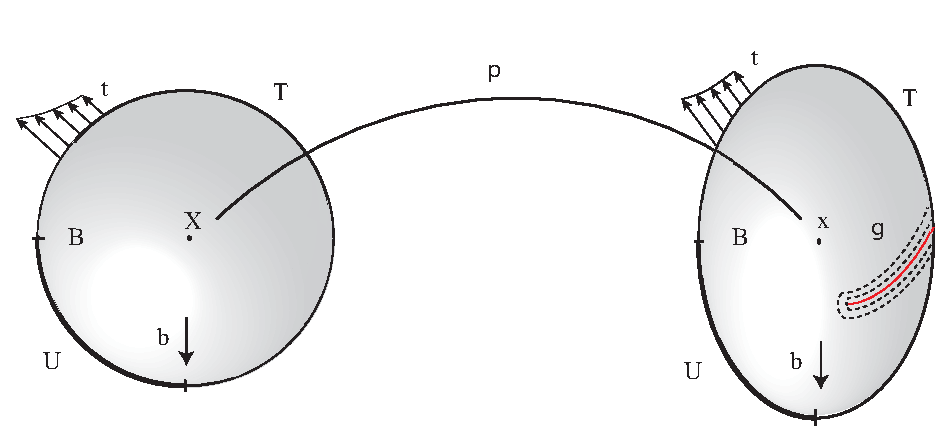
\includegraphics[height=40mm]{\slidedir/f04}
}

  \vspace{-2mm}{\tiny{Boundary value problem of diffusive fracture at large deformations}}
\end{center}

\bigskip

%Deformation gradient splitter:
%\begin{equation*}
%  \BF=\sum_{a=1}^{3} (\lambda_a^+)^d (\lambda_a^+)^{(1-d)} \lambda_a^- \Bn_a \otimes \BN_a \WITH 
%  \BF^e=\sum_{a=1}^{3} (\lambda_a^+)^{(1-d)} \lambda_a^- \Bn_a \otimes \BN_a 
%\end{equation*}
%with $\lambda_a^{\pm}=[(\lambda_a-1)\pm|\lambda_a-1|]/2+1$. 

Global energy storage functional is given as
\begin{equation*}
  E(\varphi,d)=\int_{\body} \psi(\BF,d) dV  + \int_{\body}g_c \gamma(d,\nabla d)~dV.  % \WITH  \int_{\body} \psi(\BF,d) dV = \int_{\body} \psi(\BF^e) dV
\end{equation*}
The two governing equations are
\begin{equation*}
%  \text{Div} (\BP) + \Bb =\Bzero \AND  g_c\delta_d\gamma=\frac{\partial \psi(\BF^e)}{\partial d}
  \text{Div} (\BP) + \Bb =\Bzero \quad\AND\quad  g_c\delta_d\gamma=\frac{\partial \psi(\BF,d)}{\partial d}.
\end{equation*}
%Irreversibility:
%\begin{equation*}
%  \frac{\partial \psi(\BF^e)}{\partial d} = -\sum_{a=1}^{3} \text{log}(\lambda_a^+)(\lambda_a^+)^{(1-d)} \frac{\partial \psi}{\partial \lambda_a^e} 
%  \quad \text{log}(\lambda_a^+)=0 \text{ under compression.}
%\end{equation*}

\end{frame}

